\documentclass[a4paper,oneside,article]{memoir}
\usepackage[T1]{fontenc}
\usepackage{textcomp}
\usepackage[utf8]{inputenc}
\usepackage[danish]{babel}
\usepackage[garamond]{mathdesign}
\usepackage{tikz}

\renewcommand{\ttdefault}{pcr} % bedre typewriter font
\renewcommand{\rmdefault}{ugm} % garamond

%\overfullrule=5pt

\setsecnumdepth{part}

\title{Kravspecifikation til hjemmesideanalyse  \\
       \small{Førsteårsprojekt}}

\author{ Gruppe 1:\\
  Troels Henriksen (athas@sigkill.dk)\\
  Jesper Reenberg (reenberg@kampsax.dtu.dk)\\
  Martin Dybdal (dybber@dybber.dk)\\ \\
Vejleder: Dina
}


\pagestyle{plain}

\date{\today}

\begin{document}
\maketitle

\section{Baggrund}
Når man laver en hjemmeside er det ofte fordi man gerne vil have et
budskab ud, hvad enten det er et firma eller en privatperson der står
bag. For at få sit budskab ud så effektivt som muligt bliver man nødt
til at gøre teksten man skriver så læsbar som muligt. Det er ikke altid
åbenlyst for en tekstforfatter hvor svær teksten vil være at læse for
en anden, især hvis forfatteren er vant til at skrive til en anden
målgruppe.  teksten på en del hjemmesider er derfor ikke så
tilgængelig som den kunne være.

Når man vil forfatte noget tekst er der en del der kan gå galt ---
eller i hvert fald mindske læsbarheden. Hvis man fx bruger
komplicerede ord, skriver langesætninger og laver stavefejl vil
læsbarheden falde drastisk. Man risikerer derved at budskabet man vil
sende når ud til færre mennesker.

Der er flere måder at forbedre læsbarheden af en tekst. Bl.a. har
typografi, farver og opsætning også indflydelse på hvor nem en tekst
er at læse.

\section{Formål}
For at hjælpe hjemmeside-forfattere vil vi konstruere et program der
kan analysere hjemmesider og hjælpe med at identificere passager hvor
læsbarheden ikke er i top. Programmet vil kun fokusere på selve
teksten, udseendet vil ikke blive vurderet. Hvis en hjemmeside bruger
en dårlig skrifttype, så er det en designmæssig beslutning, som vi
ikke kan vurdere positivt eller negativt.

En anden brugssituation kunne være en webmaster, som vil checke tekst
skrevet af andre på tværs af hele det website som han er ansvarlig
for.

En person i vores målgruppe er en hjemmesideskribent der er bekendt
med HTML. Personen har en professionel interessere i at teksten er
læsbar, således at vedkommende selv vil sætte sig ind i betydningen af
de udførte analysers resultater.

Det forventes også at læseren af denne kravspecifikation er bekendt
med rudimentær HTML, XML og koncepterne bag tegnindkodning.

\section{Terminologi}
Her er definitionen af nogle begreber vi bruger.
\begin{description}
\item Websted --- en samling HTML-sider placeret på samme domæne. Et
  websted indeholder én eller flere \textit{sider}.
\item Side --- en enkelt HTML-side på et websted.
\item Slemhedsfaktor --- et tal der angiver hvor svær en given side er
  at læse.
\end{description}

\section{Analyse}
Vi vil i dette afsnit prøve at fastsætte nogle uformelle målsætninger
med programmet.

Når man beder om en analyse af et helt \textit{websted} hentes
forsiden (eller en anden repræsentativ side), og hyperlinks følges med
henblik på at skabe en liste over alle sider på webstedet. Derefter
udføres en konkret tekstanalyse af indholdet på hver enkelt side.

For den enkelte HTML-side vil der blive beregnet en
\textit{slemhedsfaktor} (navn åbent for revision), et tal, der angiver
hvor svær teksten på siden er at læse. Denne faktor beregnes ud fra
LIX og FKRT-analyseresultaterne (via en algoritme som kombinerer
resultaterne som ligebyrdige, se krav 2.1.5) og vises for hver side i
analyseresultatet af hele websites, for at gøre det muligt at få et
hurtigt overblik over hvilke sider på websitet der er særligt svære at
læse. Slemhedsfaktoren skal altså ses som et redskab til at finde
undersider på webstedet der trænger til at blive kigget efter.

Det er en målsætning at analyseresultatet er let at fortolke,
f.eks. ved at visualisere resultatet ved at vise den analyserede tekst
sat med farver der angiver analyseresultatet.

Analyseresultatet består af en oversigt over hele websitet, med en
liste over undersider og et resumé af deres individuelle
analyseresultater (slemhedsfaktor, antal stavefejl, osv). Ved at
klikke på disse resuméer bringes man til analyseresultatet for en
specifik side, som indeholder mere detaljeret information, bl.a. en
liste over al tekst på siden, der er sat med farver som angiver de
enkelte sætningers sværhedsgrad. For flere detaljer, se krav 5.

\section{Prioritering}
Vi har inddelt kravene i 3 prioritets-kategorier.
\begin{description}
\item Uundværlige \textbf{(U)}, krav der skal opfyldes af en
  prototype. Krav med denne prioritet dækker uundværlig
  funktionalitet, hvis tab ville resultere i at programmet var nærmest
  ikke-funktionelt.
\item Vigtige \textbf{(V)}, krav der kan undværes, men vil resultere i
  åbenlyse mangler i programmet. Krav med denne prioritet forventes at
  være opfyldt i den endelige implementation.
\item Mindre vigtige \textbf{(M)}, krav der ikke er nødvendige for at
  programmet kan bruges, men som kunne være rare at have med i en
  senere revision. Implementationen skal altså tage højde for at disse
  krav skal kunne implementeres senere hen.
\end{description}

\section{Krav til funktionalitet}
\subsection{Krav 1: Analyse af et helt websted (U)}
Man skal kunne foretage en overordnet analyse af et helt
websted. Dvs. alle undersider (som kan nås via links fra forsiden)
skal medtages og der skal produceres information om dem (se Krav 2.1).

Hvis man eksempelvis beder om en analyse af hele diku.dk, så skal
programmet finde frem til alle undersider (diku.dk/undervisning/,
diku.dk/forskning/ osv.) og udføre en komplet tekstanalyse af hver af
disse undersider, samt producere en oversigt over alle undersiderne.

For en webmaster er det yderst relevant at udføre tekstanalyse på et
helt websted, for derefter at gribe ind på de undersider hvor det er
nødvendigt. På selv et middelstørrelses-websted kan det være
uoverskueligt at analysere hver enkelt underside manuelt.

\textit{Krav fra opgavestiller.}

\subsubsection {Krav 1.1: Respekter robots.txt (U)}
Programmet skal respekterer eventuelle robots.txt
\footnote{http://www.robotstxt.org/wc/robots.html} filer. Det skal
være muligt at slå dette fra.

Vi vil nødigt chikanere nogle ved at lade vores program crawle på
sider hvor det er uønsket. Vi vil dog heller ikke forhindre vores
program i at virke, bare fordi man ikke ønsker at blive indekseret af
søgemaskiner.

\textit{Krav fra opgavestiller.}

\subsubsection{Krav 1.2: Dybde af crawling (V)}
Det skal være muligt at angive den dybde af hyperlinks fra hovedsiden
som analyseprogrammet skal følge, hvis man sætter det til at analysere
en hel side. At sætte dybden til 0 har den effekt at kun den side man
direkte angiver til programmet (oftest websitets forside) vil blive
analyseres. Dette har den fordel at hvis man sætter den til at
analysere wikipedia.org så vil programmet ikke dø. Wikipedia.org er så
stort et websted at programmet vil kunne komme til at opbruge al
hukommelsen.

\subsection{Krav 2: Analyse af en konkret side (U)}
Man skal kunne bede om en udvidet analyse af en konkret underside.

Hvis man eksempelvis beder om en analyse af diku.dk/forskning/ skal
programmet foretage forskellige tekstanalyser af sidens
tekst. Begrebet ``sidens tekst'' dækker ikke alene over brødtekst,
dvs. tekst forefindende direkte mellem tags i sidens krop, men også
teksten som udgør værdien til \texttt{title}, \texttt{summary},
\texttt{alt} og lignende attributter.

\textit{Krav fra opgavestiller.}

\subsection{Krav 2.1: Analysemetoder}
Vi vil kunne understøtte de følgende analysemetoder til at analysere
teksten på en side.

\subsubsection{Krav 2.1.1: Læsbarhedsindeks, LIX (U)}
Programmet skal kunne udregne lixtal.

\subsubsection{Krav 2.1.2: Flesch-Kincaid Readability Test (FKRT) (V)}
Programmet skal kunne udføre Flesch-Kincaid Readability Test.

\subsubsection{Begrundelse for krav 2.1.1 og 2.1.2}
De to analysemetoder supplerer hinanden godt, idet LIX primært er
baseret på ordlængde, hvorimod FKRT også tager sig af
sætningslængde. Sammen giver de et rimeligt billede af tekstens
sværhedsgrad. Det er endnu ikke besluttet om resultatet for de to
analysemetoder skal kombineres eller vises separat fra hinanden.

\subsubsection{Krav 2.1.3: Stavekontrol (V)}
Programmet skal kunne finde stavefejl. Som udgangspunkt skal
programmet kun kunne stavefejl i danske tekster (se krav 2.1.3.1).

Stavekontrollen vil ikke indgå i beregningen af slemhedsfaktoren, men kun
blive brugt til at vise stavefejl da dette vil være alt for
svært at håndtere (fx hvis en dansk side indeholder mange
engelske termer).

\subsubsection{Krav 2.1.3.1: Flere sprog (M)}
Programmet skal kunne udvides til et arbitrært antal sprog (defineret
ved deres sprogkode).

\subsubsection{Krav 2.1.4: Gentagne ord (V)}
Programmet skal kunne finde gentagne ord.
Denne analyse skal heller ikke påvirke slemhedsfaktoren.

\subsubsection{Krav 2.1.5: Beregning af slemhedsfaktor (V)}

For hver enkelt side beregnes der et entydigt tal, der angiver sidens
tekstmæssige sværhedsgrad. Dette tal betegnes sidens
\textit{slemhedsfaktor}. LIX og FKRT-analyser resulterer i en talværdi
der angiver tekstens sværhedsgrad. Da disse talværdier ikke befinder
sig på samme skala, er det nødvendigt at finde en vægtningsfaktor som
kan sikrer at en af de to algoritmer ikke vil have en uforholdsmæssigt
stor indflydelse på slemhedsfaktoren. Denne vægtningsfaktor er endnu
ikke kendt, men vil bestemmes ved at udføre LIX og FKRT-analyser på en
mængde repræsentative tekster og sammenligne talresultaterne

\subsection{Krav 2.2: Analyse baseret på HTML-tags. (M)}
Den semantiske information som HTML-tags angiver skal bruges til at
påvirke vægtningen af de andre analyser. Dette omfatter de følgende
underkrav.


\begin{itemize}
\item Overdreven brug af \texttt{em} og \texttt{strong} kan påvirke
  tekstens læsbarhed. Samtidigt indeholder sætninger med disse tags
  måske også vigtigere/mindre vigtige end andre, og bør derfor
  resultere i en anden vægtning af deres LIX og
  FKRT-analyseresultater.
\item Overskrifter (\texttt{hN}-tags) skal vægtes anderledes end
  resten af teksten, eller evt. totalt ignoreres. Overskrifter kan
  have en større (eller mindre) betydning for tekstens samlede
  læsbarhed end deres tekstmængde umiddelbart ville lede en til at
  tro.
\item Der skal ikke angives stavefejl for ord i \texttt{acronym} og
  \texttt{abbr} tags, da disse angiver at ordene er forkortelser.
\item Tekst, angivet som et sprog (via \texttt{lang}-tagget) som ikke
  er understøttet, skal ikke stavekontrolleres.
\item Tekst i \texttt{q} eller \texttt{blockquote}-tags
  (dvs. citationer) skal ikke analyseres, men dog stavekontrolleres,
  da det ikke formodes at disse kan skrives om.
\item Visse tags, som f.eks. \texttt{kbd}, \texttt{var}, og
  \texttt{code} angiver at teksten ikke indeholder almindelig tekst,
  og derfor ikke skal analyseres.
\item \texttt{bdo}-tagget kan bruges til at angive, at teksten skal
  skrives fra højre mod venstre (eller omvendt). I dette tilfælde skal
  bogstaverne i teksten vendes om før der udføres stavekontrol.
\end{itemize}

Der tages forbehold for senere tilføjelse af andre tags der skal
specialbehandles.

\subsection{Krav 2.3: Konfiguration af analyse (M)}
Programmet skal gøre det muligt at angive hvor omfattende en analyse
der skal foretages og lade brugeren indstille de enkelte
analysemetoder. Man skal kunne indstille:

\begin{itemize}
\item Hvilke analyser der skal udføres.
\item Hvilke dele af siden der skal medtages, baseret på
  HTML-elemen\-ter\-nes \texttt{id} og \texttt{class}-attributter. Så man
  fx kan udelukke brugerkommentarer fra analysen.
\end{itemize}

Det kan fx være muligt at angive hvilke tjek der skal foretages (fx
stavekontrol eller lix-beregning) og hvilke dele af siden der
skal medtages i analysen. Fx skal citater og tabel-data måske
udelades. Man kan også forestille sig at man vil ændre på hvordan
overskrifter skal vægtes i analysen. 

\section{Krav til interface}

\subsection{Krav 3: Kommandobaseret interface (U)}
Programmet vil være udformet som et kommandolinjeværktøj, og
interfacet vil bestå af kommandolinjeparametre. Programmet vil som
minimum tage en URL som parameter, og vil derudover understøtte
parametre til at kontrollere programmets specifikke opførsel -
f.eks. de i krav 1 og 2 nævnte to forskellige
analysefremgangsmåder. At implementere interfacet som et
kommandolinjeprogram sikrer at vi har mere tid til at implementere
effektive analysemetoder, og at det vil være overkommeligt at lave et
grafisk interface baseret på kommandolinjeværktøjet senere hen.

\subsection{Krav 4: Resultater i HTML-format. (V)}
Programmet skal generere HTML-filer der viser resultatet af en
analyse. Der genereres en index-fil der fungerer som indgang til
resten af analysen. Dette index indeholder en liste over alle de
undersider der er blevet analyseret, samt et resumé af deres
analyseresultat (f.eks. deres slemhedsfaktor - evt. er listen over
undersider sorteret efter denne slemhedsfaktor). Der bliver også
genereret en HTML-fil for hver analyseret underside - denne fil
indeholder en detaljeret analyse, bl.a. bestående af al tekst på
siden, hvor hver sætning er sat med farver alt efter hvor svær den er
at læse. På disse sider fremgår de konkrete LIX og FKRT-resultater
også, i stedet for blot at vise slemhedsfaktoren. Samtidigt fremgår
resultatet af stavekontrollen også. Fra index-sidens liste over
undersider går der links til disse HTML-resultat-filer.

Dette er for at kunne lave mere avanceret visualisering af
analyseresultatet. At generere HTML-filer kan også lette
implementationen af et eventuelt senere web\-appli\-kations-baseret
interface.

\section{Krav til implementationen}

\subsection{Krav 5: Platform}
Programmet skal kunne køre på typiske GNU-baserede Linux
maskiner. Dette er for at minimere antallet af systemkonfigurationer
som skal testes.

\subsection{Krav 6: Håndtering af HTML/XHTML (U)}
Programmet skal håndtere sider der overholder de gældende HTML
og XHTML standarder. Dog vil vi begrænse mængden af XHTML der skal
understøttes. Vi vil kun implementere den delmængde af XML der er
løftet næsten direkte fra SGML, hvilket er tilstrækkeligt til langt
den største part af XHTML-dokumenter.

Dette krav betyder at en side der ikke overholder standarderne
ikke altid vil blive analyseret korrekt, dog kan programmet prøve at
gætte på hvad der menes hvis der eksempelvis mangler et afsluttende
tag (fx \texttt{</tr>}).

Dette betyder også at der skal tages speciel hånd om nogle tags der
kan have indhold der kan ødelægge parsingen (eksempelvis
\texttt{<style>}, \texttt{<script>} og HTML-kommentarer).

\subsubsection{Krav 6.1: Encoding}

Kun sider indkodet i ASCII eller Moscow ML's indbyggede indkodning
(sandsynligvis ISO-8859-1/Latin-1 på de fleste maskiner)
understøttes. Det kunne være rart også at understøtte UTF-8, og bruge
den indkodning som HTML-siden ønsker, men af simplicitetshensyn er
dette ikke et konkret krav. Dette krav er for at holde fokus, da
implementationen af indkodnings-håndtering hurtigt kan lægge beslag på
en tidsmængde som er ude af proportioner med hvad en sådan
indkodnings-understøttelse ville give os af fordele.

\section{Illustration af afhængigheder}
\textit{For overskuelighedens skyld er krav uden afhængigheder
  udeladt.}


\vspace{0.3cm}


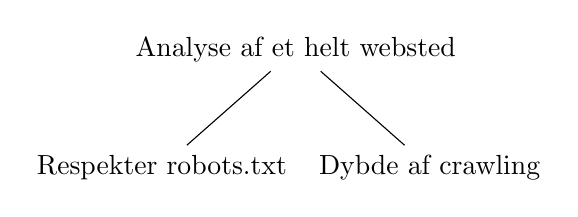
\begin{tikzpicture}
    \tikzstyle{level 1}=[sibling distance=34mm]
    \tikzstyle{level 2}=[sibling distance=22mm]

    \node {Analyse af et helt websted}
        child { node {Respekter robots.txt} }
        child { node {Dybde af crawling} }
    ;
\end{tikzpicture}

\vspace{0.3cm}

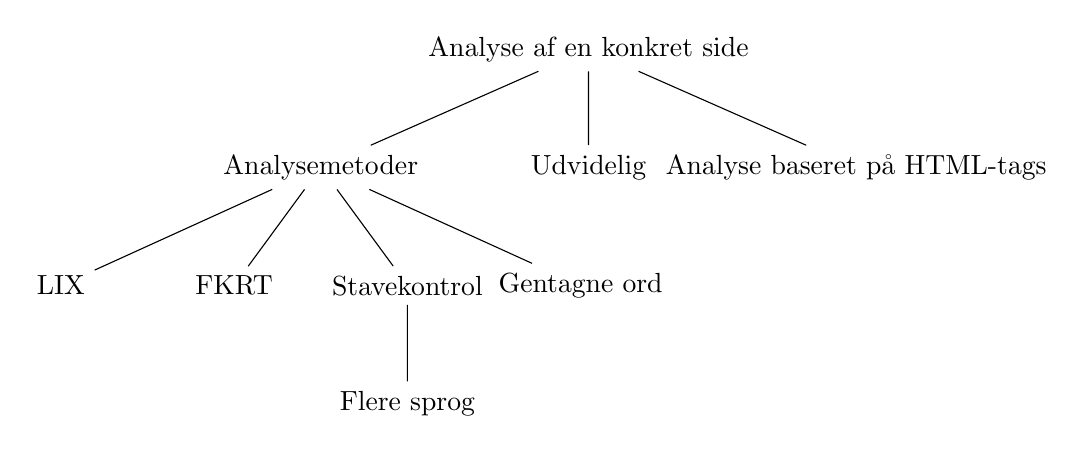
\begin{tikzpicture}
    \tikzstyle{level 1}=[sibling distance=34mm]
    \tikzstyle{level 2}=[sibling distance=22mm]

    \node {Analyse af en konkret side}
        child
        { 
          node {Analysemetoder}
          child { node {LIX} }
          child { node {FKRT} }
          child { node {Stavekontrol}
                  child { node {Flere sprog} }
          }
          child { node {Gentagne ord} }
        }
        child { node {Udvidelig}}
        child { node {Analyse baseret på HTML-tags}}
    ;
\end{tikzpicture}

\end{document}
